\chapter{conclusiones} \label{Conclusiones}

\section{Resultados y pautas de la actividad.} \label{sec:resultado}
\subsection{Resultado.} \label{subsec:resultado}
Éste es el resultado del proyecto editado.

\begin{figure}[H]
\centering
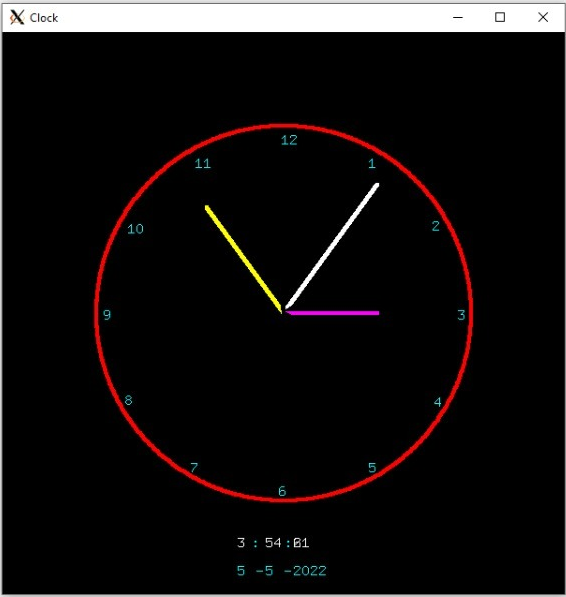
\includegraphics[width=0.4\textwidth]{../img/chapter03/7.png}
\caption{Resultado del proyecto}
\label{fig:resultado}
\end{figure}

La diferencia que se puede ver aquí,es que, ya que WSL (por lo menos en su versión 1) no tiene capacidad de ejecutar gui nativamente, por lo que tuve que usar un servidor para que pudiera correr la gui de la aplicación desde WSL.

\subsection{Pautas del ejercicio.} \label{subsec:pautas}
Luego de lo mostrado alrededor de los capítulos, y de ilustrar el resultado obtenido en el apartado \ref{subsec:resultado}, vamos a disponer de responder unas pautas que nos deja el ejercicio.

\begin{myquote}
¿Funciona bien tu programa?
\end{myquote}

como vimos en la figura \ref{fig:resultado}, el reloj funciona correctamente.

\begin{myquote}
¿Qué fallos existen?
\end{myquote}

Como tal, no se encontraro errores en la primera versión del archivo donde no hace uso de la programación orientada a objetos, sin embargo, por la dificultad de poder visualizar el resultado por mí mismo (porque el proceso es muy lento por el uso de XLaunch para windows, la primera versión me la revizó un compañero de la universidad, a quién nombraré en el apartado de agradecimientos).

\chapter{Recursos}
\href{https://pharos.sh/breve-introduccion-a-opengl-en-python-con-pyopengl/}{https://pharos.sh/breve-introduccion-a-opengl-en-python-con-pyopengl/}

\href{https://codingshiksha.com/python/python-3-opengl-script-to-build-3d-digital-analog-clock-using-pyopengl-library-gui-desktop-app-full-project-for-beginners/}{https://codingshiksha.com/python/python-3-opengl-script-to-build-3d-digital-analog-clock-using-pyopengl-library-gui-desktop-app-full-project-for-beginners/}

\href{https://yewtu.be/watch?v=9rmxMUyFcj4}{https://yewtu.be/watch?v=9rmxMUyFcj4}



\chapter{Agradecimientos}
Mi especial agradecimiento a mi compañero \textbf{Sebastian Steffen Castañeda Castillo} por la ayuda y colaboración para ayudarme a comprobar el funcionamiento del proyecto debido que a causas técnicas, no pude comprobarlos por mí mismo.

De igual manera, agradecer a todos aquellos compañeros que, de forma desinteresada, me han aportado con sus conocimientos el poder llevar adelante éste laboratorio.



